% !TEX root = ../../../semexp-thesis.tex

\section{Domain Model}
\label{sec:semtex/model}

We describe our domain model of semantic technologies for programming semantic searches and conversational agents.

\subsection{Semantic Search}
\label{sec:semtex/model/search}

To model semantic search in the context of the Squeak ecosystem, \semtex defines the central class \code{SemanticCorpus} as a specialization of the \code{Set} class from the Collections package~(\cref{fig:semtex/model/search}).
This class extends the responsibilities of a regular collection for containing any number of (domain) objects with those of a vector store for searching and filtering objects based on document embeddings.

\begin{figure}
	\centering
	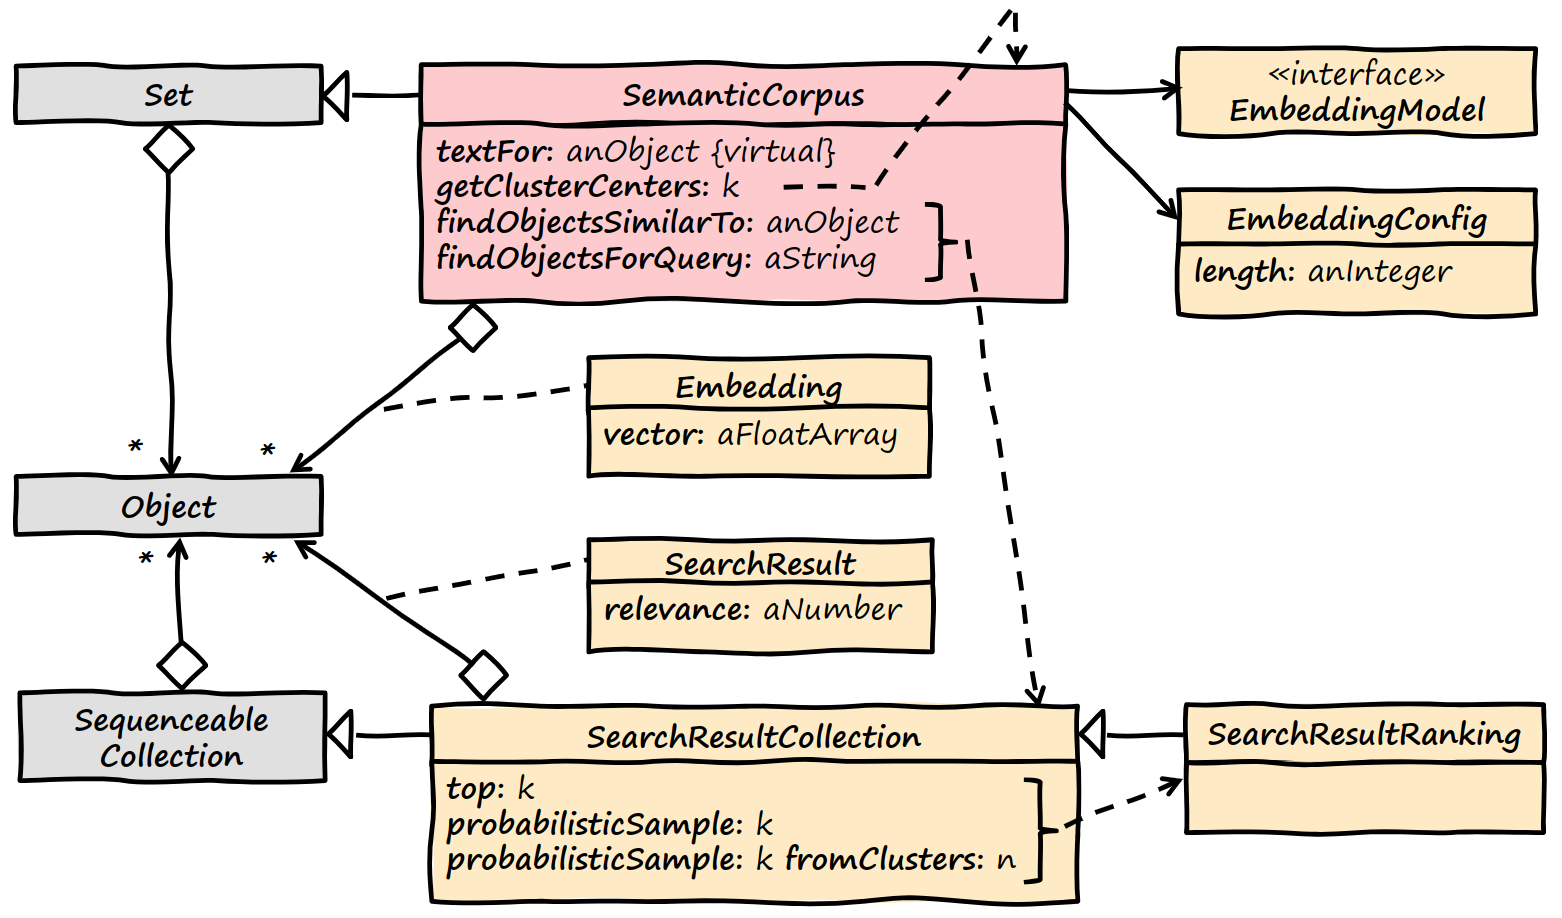
\includegraphics[width=\textwidth]{a_semtex/model/search.png}
	\caption[TODO]{
		TODO
	}
	\label{fig:semtex/model/search}
\end{figure}

For each object, the corpus computes and stores an \code{embedding} vector that is represented by a \code{FloatArray}, allowing for efficient comparison, memory consumption, and serialization.
To compute embeddings, the corpus is provided with a \code{SemanticEmbeddingModel} (which may be implemented by different providers, see \cref{sec:semtex/providers}) and a \code{SemanticEmbeddingConfig} for controlling the embedding properties such as the length of embedding vectors.
To embed non-textual object elements, the corpus can be provided with a \emph{text conversion} function through composition or specialization (e.g., by registering an evaluable block or overriding a method)\footnote{Currently accessible through \code{SemanticPluggableCorpus}.}.

The semantic corpus provides methods for searching objects that are \emph{similar} to a reference object or to a natural-language \emph{query} string.
For each search, it answers a \code{SemanticSearchResultSet}, which contains a \emph{relevance score} for each object in the corpus\footnote{At the time of writing, these classes have not yet been extracted from the \code{SemanticCorpus} in our public implementation.}.
A result set can be \emph{ranked} into a \code{SemanticSearchResultRanking} of a finite length using the different ranking methods discussed in \cref{sec:suggestions/ranking}, such as top-k selection or probabilistic sampling.
Additionally, the semantic corpus also supports cluster-based selection of representative objects.

%\begin{example}
%	A programmer wants to find classes in the system that implement means for semantic search.
%	For this, they can semantically search all classes based on their names:
%
%	\begin{multicode}
%		corpus := self systemNavigation allClasses \newline
%		\null\qquad	collect: \#name \newline
%		\null\qquad	as: SemanticCorpus. \newline
%		results := corpus findObjectsSimilarToQuery: \textquotesingle semantic search database\textquotesingle. \newline
%		ranking := results top: 5. \newline
%		ranking \printit{a SemanticSearchResultRanking(\allowbreak\#SemanticCorpus->0.45 \#SemanticAgent->0.433 \#SemanticAgentParser->0.412 \#WordNet->0.412 \#SemanticMathAgent->0.402)}
%		% todo: introduce printit notation anywhere?
%	\end{multicode}
%
%	To further improve the quality of the search results, the programmer can also include the comment of each class into the embeddings.
%	For this, they use some additional convenience methods for converting domain objects into text and computing a ranking directly:
%
%	\begin{multicode}
%		self systemNavigation \n
%		\t	semanticWithTitle: \#name \n
%		\t	content: \#comment \n
%		\t	findTopObjects: 5 \n
%		\t	similarToQuery: \textquotesingle semantic search database\textquotesingle{} %\n
%		\printit{a SemanticSearchResultRanking(\allowbreak\#SemanticCorpus->0.533 \#SemanticHelpSearchTopic->0.442 \#SemanticText->0.385 \#SemanticAgentParser->0.364 \#SemanticMathAgent->0.338)}
%	\end{multicode}
%\end{example}

\begin{example}
	A programmer wants to find classes in the system that implement means for semantic search.
	For this, they can create a semantic corpus of all classes based on their names and comments, perform a search, and rank the results:

	\begin{multicode}
		corpus := self systemNavigation allClasses \newline
		\null\qquad	asSemanticCorpusWithTitle: \#name \newline
		\null\qquad	content: \#comment. \newline
		results := corpus findObjectsSimilarToQuery: \textquotesingle semantic search database\textquotesingle. \newline
		ranking := results top: 5. \newline
		ranking \printit{a SemanticSearchResultRanking(\allowbreak\#SemanticCorpus->0.533 \#SemanticHelpSearchTopic->0.442 \#SemanticText->0.385 \#SemanticAgentParser->0.364 \#SemanticMathAgent->0.338)}
		% todo: introduce printit notation anywhere?
	\end{multicode}
\end{example}

\subsection{Conversations}
\label{sec:semtex/model/conversations}

To support text generation and machine reasoning, we integrate different conversational LLMs into \semtex.
For this, the framework defines a \code{SemanticConversation} class~(\cref{fig:semtex/model/conversation}).
A conversation contains a number of \code{SemanticMessage}s each of with is specified with a \code{role} (either system, user, or assistant) and a \code{text}.
A programmer can set up a conversation with a sequence of initial messages, such as a system message for providing instructions and a user message for the first question of the user, and ask the conversation to \code{complete} itself, which will request the (stateless) LLM and append a new generated assistant message to the conversation.

\begin{figure}
	\centering
	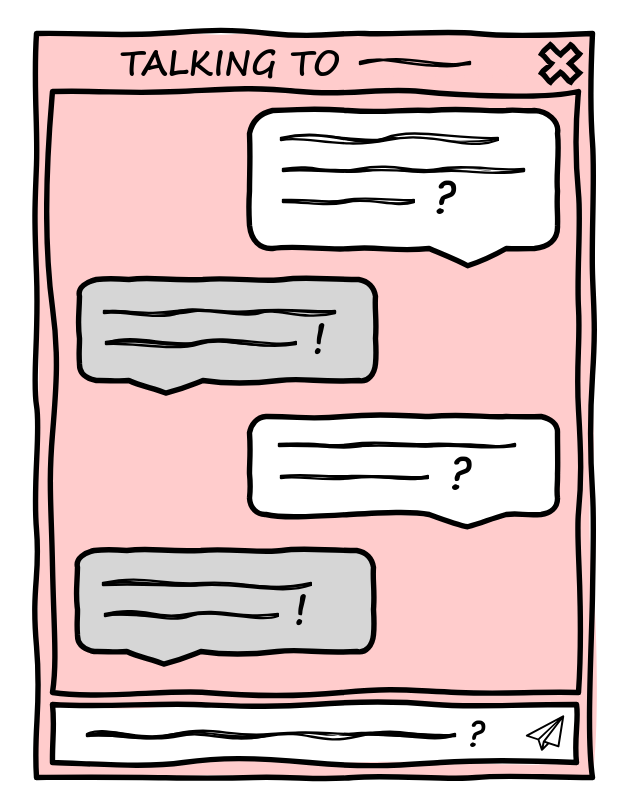
\includegraphics[width=\textwidth]{a_semtex/model/conversation.png}
	\caption[TODO]{
		TODO
	}
	\label{fig:semtex/model/conversation}
\end{figure}

To allow for the construction of agents, the conversation can also be equipped with a \code{SemanticFunctionSpec} that provides one or multiple \code{SemanticFunction}s.
Each function has a name, can specify an optional list of arguments and their constraints as well as a description, and contains an action object (e.g., a block).
When the LLM is invoked, it can issue one or multiple \code{SemanticFunctionCall}s based on the function specification as part of the generated assistant message.
The conversation automatically resolves these function calls by \code{call}ing each issued function with the generated arguments, storing the result in a new \code{SemanticFunctionMessage}, and providing all function messages to the LLM in another request, which uses the results for generating the next assistant message.

Analogously to semantic corpora, each conversation is configured through a \code{SemanticConversationModel} reference and a \code{SemanticConversationConfig} for controlling the generation behavior, such as the model temperature or the maximum number of generated tokens.

\begin{example}
	A programmer wants to create a chatbot that can retrieve the current time and date.
	For this, they define a conversation with an appropriate configuration for the LLM, define the necessary functions, and provide the question of the user:

	\begin{multicode}
		SemanticConversation new \n
		\t	withConfigDo: [:config | \n
		\t	\t	config temperature: 0.2]; \n
		\t	addFunction: \#getTime action: [Time now]; \n
		\t	addUserMessage: \textquotesingle What time is it?\textquotesingle; \n
		\t	getAssistantMessage \printit{\textquotesingle The current time is 13:59.\textquotesingle}
	\end{multicode}
\end{example}

Additionally, \semtex supports the construction of class-based agents by providing the base class \code{SemanticAgent} which users can specialize to provide custom instructions and functions.
The \code{SemanticAgent} class provides a custom DSL (domain-specific language) for specifying a function signatures with its arguments, their constraints, and their descriptions through method pragmas.
The agent class offers support for automatically dispatching function calls and handling errors during function calling.

\begin{example}
	A programmer wants to build a chatbot that can access the running Squeak image to assist the user.
	To achieve this, they create a subclass of \code{SemanticAgent}, initialize the conversation, and define an \code{\#eval:} method:

	\begin{multicode}
		SemanticAgent subclass: \#SemanticSqueakAgent \n
		\t	instanceVariableNames: \textquotesingle\textquotesingle \n
		\t	classVariableNames: \textquotesingle\textquotesingle \n
		\t	poolDictionaries: \textquotesingle\textquotesingle \n
		\t	category: \textquotesingle SemanticText-Model-Agents\textquotesingle \n
		\n
		SemanticAgent>>initializeConversation: aConversation \n
		\t	super initializeConversation: aConversation. \n
		\t	aConversation addSystemMessage: \textquotesingle You are a Squeak/Smalltalk assistant.\textquotesingle. \n
		%\t	aConversation addAssistantMessage: \textquotesingle Hi, how can I help you?\textquotesingle. \n
		\n
		SemanticAgent>>eval: aString \n
		\t	\textquotedbl Evaluate a Smalltalk expression in the running Squeak image.\textquotedbl \n
		\t	<function: eval( \n
		\t	\t	expression: string \textquotedbl %examples: \n
		%\t	\t	- \textquotesingle DateAndTime now\textquotesingle \n
		%\t	\t	- \textquotesingle| collection | collection := 1 to: 10. collection inject: 0 into: [:a :b | a + b]\textquotesingle \n
		%\t	\t	\textquotedbl \n
		e.g. \textquotesingle (8 nthRoot: 3)-1\textquotesingle\textquotedbl \n
		\t	)> \n
		\t	\textasciicircum{} Compiler evaluate: aString
	\end{multicode}

	Finally, the programmer invokes the agent:

	\begin{multicode}
		SemanticMathAgent makeNewConversation \n
		\t	addUserMessage: \textquotesingle how many windows are open\textquotesingle; \n
		\t	getAssistantReply \printit{\textquotesingle You currently have 138 open windows in your Squeak environment.\textquotesingle}
	\end{multicode}
\end{example}
% todo: reconsider syntax highlighting
